\section{Approaches}
\label{cp5:approaches}

\gm{Perhaps you could consider a structure for this 
chapter that has: 1) Problem Definition (which is the 'all approaches
below' 2) Baseline 3) Approaches. The reason is to try to make
it clear what is a baseline and what are new proposed
approaches. Let's discuss.}

In this section, we detail three approaches to automatically identify text that is relevant to a particular software task.
These approaches encompass lexical similarity, word semantics, and frame semantics.


% \gm{Argument below will need specific references back to earlier chapters (eventually).} 
All approaches take a task and a pertinent artifact as inputs and output the sentences 
that are most likely to contain information that assists a developer in completing their task. 
To determine how many sentences an approach should identify, we consider that 
no more than 20\% of the content in the artifacts in the
 \acs{DS-synthetic} and the \acs{DS-android} corpora are deemed relevant to a task (\red{Chapter~\ref{}}), which, on average, accounts for 8.93 sentences (\red{Chapter~\ref{}})
 and we approximate these values to identifying a target number of 10 sentences per input task-artifact. 
Our decision to output a certain number of sentences regardless of the approach is to have an easy framework for their comparison (Section~\ref{cp5:evaluation}).


\subsection{Lexical Similarity}

As a baseline, we investigate if the sentences that are lexical similar
to a task are more likely to contain information relevant to that task. \gm{Need argument why this is a good baseline.}


We use Vector Space Model (VSM)~\cite{Salton1975vsm} from Information Retrieval~\cite{Manning2009IR}
to compute the lexical similarity between the sentences within a pertinent artifact and a task. 
VSM represents both a task and individual sentences within an artifact as vectors of term weights,
where the weight of a term
can be computed using a Term-Frequency Inverse-Document-Frequency scheme (\textit{tf.idf})~\cite{Manning2009IR}. 
Once we obtain vector representations $t$ and $s$ 
for an input task and an arbitrary artifact sentence, 
their lexical similarity can be computed 
using the cosine similarity between their vectors, as Equation~\ref{eq:lex-sim} shows:



\begin{equation}
    cos(t,s) = \frac{t^Ts}{\|t\| \|s\|}
    \label{eq:lex-sim}
\end{equation}
\smallskip

By ranking the sentences in an artifact according to their similarity scores, i.e., from highest to lowest,
we can  select the top-n sentences as the ones relevant to an input task.

\gm{This section likely needs to provide a direct definition
of document in terms of artifacts.}

% ------------------------------------------------


\subsection{Word Semantics}


Language models \rev{represent} the semantics of words based on the context in which words appear~\cite{harris1954distributional}.
They allow a more ``human-like reasoning'' even when words are lexically different, which 
motivates investigating whether we can identify task-relevant text by semantically matching the text in a pertinent artifact to the text in a task.



We first describe how we use language models to automatically identify task-relevant text, and then
detail how we use a baseline model \gm{I think this overloads
the word baseline} \art{will rephrase it} and 
a state-of-the-art model to automatically identify task-relevant text.
For an introduction of general concepts behind language models, please refer to~\cite{zhang2021deep-learning}.

\subsubsection{Background}

% introduce language models
A core concept of a language model is Harris' distributional hypothesis~\cite{harris1954distributional}, which states that words that appear in a similar context tend to have similar meanings.


A language model exploits this hypothesis by building continuous vector representations, namely \textit{word embeddings}, for each of the words in a text corpus.
For that, it requires a significantly large number of sentences so that
the model associates similar vector embeddings to words that are similar in meaning~\cite{Ye2016}. 


% Overview of baseline model
\smallskip
\begin{hangparas}{.0in}{0}
     \textit{ Skip-gram model.} One common challenge to language models is that they need to learn word vector representations that are good at predicting the nearby words at low computational costs, e.g., the time needed to train a model, the model size, etc.
    The \textit{Skip-gram} model~\cite{Mikolov2013}, proposed by Mikolov et al., addresses such challenges using simple yet efficient training procedures. As Figure~\ref{fig:skip-gram-example} illustrates, the model learns vector representations by \textit{(i)} looking at the $n$ words that preceded and succeed word $w_t$
     as positive training examples, and by \textit{(ii)} randomly sampling words that do not appear in the same context as negative training examples. Empirical results have shown that negative sampling allows for an accurate model able to handle noise data and that 
     the vector representations provided by the model could be used to improve many natural language processing tasks~\cite{mikolov2013efficient}.
\end{hangparas}

\begin{figure}[H]
    \centering
    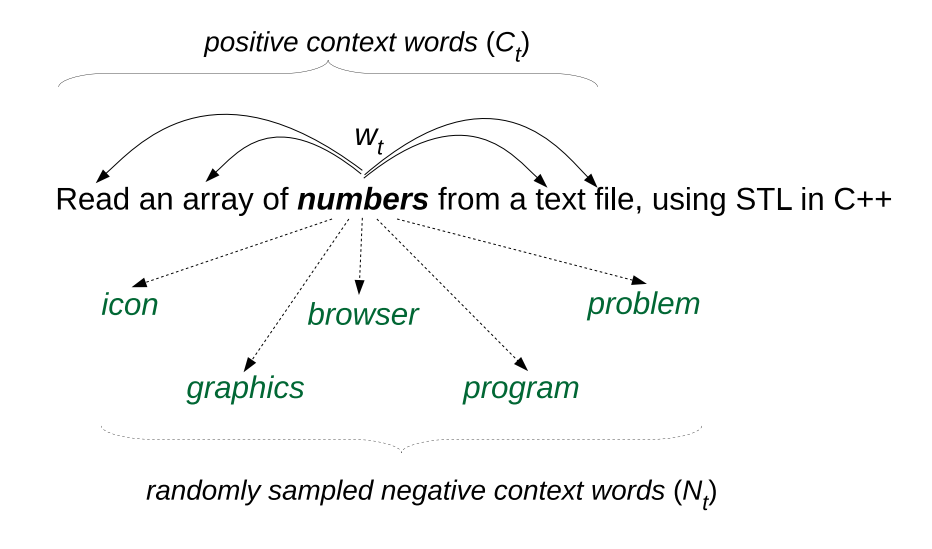
\includegraphics[width=.65\linewidth]{fig/cp5/ye-skip-gram-example}
    \caption{Positive and negative training examples in the Skip-gram model. Figure originally from~\cite{Ye2016} \gm{Unfortunately you can't use this diagram without permission if it is from a published text.} \art{Sorry. I'll update the figures}}
    \label{fig:skip-gram-example}
\end{figure}


Using the skip-gram model, one can identify that words $t$ and $s$ are semantically similar 
computing the cosine similarity between their corresponding word embedding representations, i.e., $w_t$ and $w_s$:



\begin{equation}
    cos(w_t,w_s) = \frac{w_t^Tw_s}{\|w_t\| \|w_s\|}
    \label{eq:word-sim}
\end{equation}




% Overview of state-of-the-art model
\medskip
\begin{hangparas}{.0in}{0}
     \textit{BERT model.} Context in the Skip-gram model refers to the positive/negative examples used during the model's training procedures; this, however, does not allow the model to disambiguate words based on their surrounding text. In other words, a Skip-gram model will have a single vector representation for the word \textit{company} even when it can have different meanings, i.e., a business organization or being with someone. In contrast, state-of-the-art models, such as \textit{BERT}~\cite{Devlin2018Bert}, provide different representations for the same word based on the sentence in which a word appears.
    This additional layer allows for more complex operations, such as word disambiguation \red{ref}.
\end{hangparas}



BERT also addresses tasks that need to understand relationships between sentences, which is a task not directly captured by language modeling~\cite{Devlin2018Bert}. \gm{I am struggling with the
idea that tasks 'need' to understand relationships between sentences. More explanation is likely needed.}
To capture sentence relationships, BERT training procedures consider both next word prediction---as in any language model---and also next sentence prediction, i.e., given a pair of sentences $A$ and $B$, the model 
is trained to predict the likelihood that sentence $B$ succeeds (or not) sentence $A$ (Figure~\ref{fig:BERT}). 


\art{Perhaps, one way to explain this is: 
\begin{enumerate}
    \item word2vec cosine-sim is one way to identify that a task-artifact sentence pair is semantically similar and, because of that, the artifact sentence is relevant to the task
    \item BERT does the same but rather than using cosine-sim it uses an attention function~\cite{Vaswani2017attention}. It will take a task-artifact sentence pair and indicate whether the artifact sentence is relevant for that task
    \item Cosine-sim weights all words in a task-artifact sentence pair equally. Attention will find that certain words contribute more.
\end{enumerate}
}





\begin{figure}
    \centering
    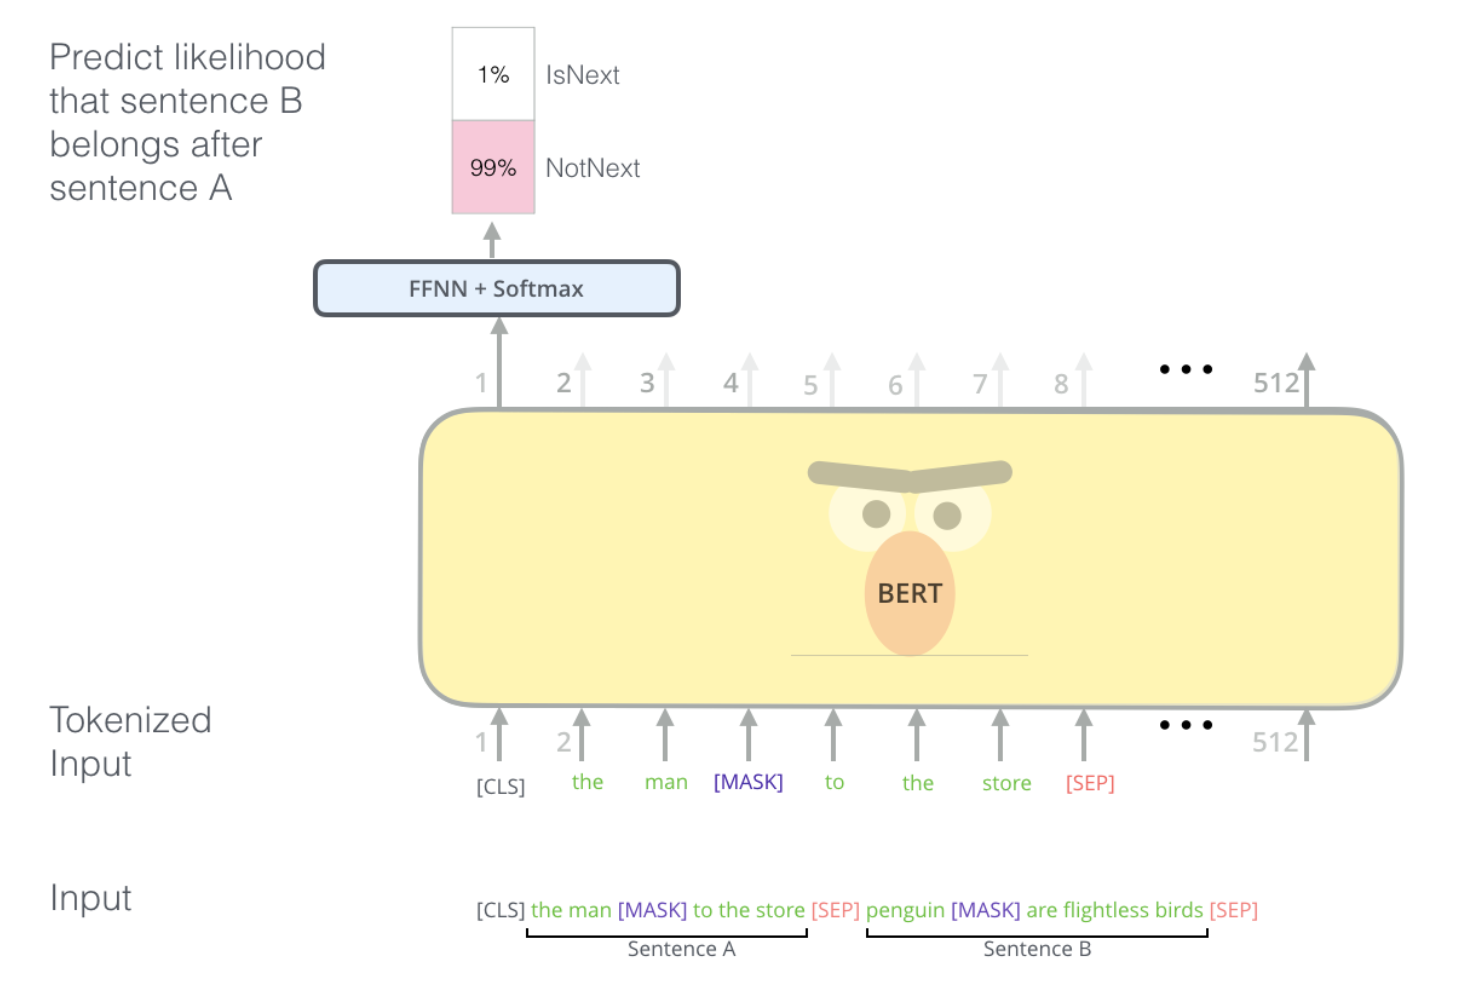
\includegraphics[width=.75\linewidth]{fig/cp5/BERT}
    \caption{BERT next sentence prediction training procedures. Figure originally from~\cite{jay-alammar-bert} \gm{Same issue with re-using Figure} \art{TODO: update}}
    \label{fig:BERT}
\end{figure}



Since BERT addresses both next word prediction and next sentence prediction, the model can be used for several
word semantics and sentence relationship tasks such as  ours, i.e., determine the relevance of a sentence within an artifact based on a second sentence representing a task description. \gm{How is
this sentence prediction? Is there precendence for using
BERT on two different artifacts (i.e., the task description
can be considered an artifact or document.)}


\art{Cleland-Huang's group have used BERT to associate requirement docs to python docstrings~\cite{Lin2021}; it has also been used to build correlations between
 app reviews and requirements docs~\cite{Araujo2021}}

% ------------------------------------------------


\subsubsection{Semantic Similarity}
\label{cp5:skip-gram}

\gm{Is this still part of background? There needs to be
some more walking the reader through where this part is
going. Maybe introduction some nomenclature for
actual approaches you are introducing. Let's discuss.}

Similar to lexical similarity,  we investigate if the sentences with the highest semantical similarity are most likely to contain information relevant to the input task.


To compute the semantic similarity between the sentences within a pertinent artifact and a task,
we use the Skip-gram model~\cite{Mikolov2013} with word embeddings specifically trained for the software engineering domain~\cite{Efstathiou2018}.
Since word embeddings provide vector representations at the word level, we follow Conneau et al.'s guidelines~\cite{conneau2018} 
and compute vector representations for an entire sentence by averaging the sum of the word embeddings in that sentence.


Provided that we have embeddings $w_t$ and $w_s$ for the text 
of an input task and an arbitrary artifact sentence, 
their semantic similarity can also be obtained 
using the cosine similarity. In turn, we can select the top-n sentences
with the highest semantical similarity as the ones likely relevant to an input software task.


% ------------------------------------------------


\subsubsection{Artifact-Task Sentence Relationships}
\label{cp5:bert}


We use the BERT model~\cite{Devlin2018Bert} to establish relationships between artifact and task sentences pairs and determine 
the sentences within an artifact that most likely contain information relevant to the task.


Since BERT requires training procedures, we start with an already pre-trained model, namely BERT\textsubscript{uncased}, and we tune it to  identifying task-relevant text.
\gm{Is BERT\textsubscript{uncased} something from elsewhere?}
As done by several other studies (e.g., ~\cite{Chaparro2017, fucci2019, Petrosyan2015}), we use standard cross-validation techniques to ensure  that no data used for evaluation is also used
during the model's training procedures. More specifically, we use 10-fold cross-validation with 70\%, 20\% and 10\% splits for training, validation and testing. 


The model outputs probability scores indicating the likelihood of a sentence being relevant to an input task.
We select the top-n sentences predicted by the model as relevant.



% ------------------------------------------------


\subsection{Frame Semantics}


\art{I still need to check frames based on the tasks in \acs{DS-synthetic}, so there might be updates to this section. }


Given our analysis of relevant sentences in the \acs{DS-synthetic} corpus, we pose that 
sentences with certain meanings, such as the ones that provide instructions on using an entity to achieve some goal,
are sentences that a developer would first pay attention to when inspecting a software artifact and thus, they are more likely to contain task-relevant information. \gm{Will need more on why
this hypothesis.}



We implement this hypothesis as a post-filtering step~\cite{Manning2009IR} applied to the lexical similarity and word semantics approaches.
Given a set of sentences returned by an approach, 
we use the \textit{SEFrame} tool~\cite{marques2021} as a proxy to the sentence's meaning,
checking if the semantic frames obtained by the tool appear in a set of frames drawn from  sentences annotated as relevant in the \acs{DS-synthetic} corpus.





% ------------------------------------------------


\subsection{Approaches Summary}


Table~\ref{tbl:approaches-summary} bundles the approaches that we explore.
The table provides a short identifier for each approach, identifies the research topic that serve as a basis for each approach and provides a short description for them. From now on, we refer to each approach according to their short identifier.

\gm{Isn't there multiple SEframes approaches?}


\begin{table}[H]
\centering    
\begin{scriptsize}
\begin{threeparttable}
\rowcolors{2}{}{lightgray}    
\begin{tabular}{lll}

% \hline

% \multicolumn{2}{c}{\textit{No lock screen controls ever}}  \\



\textbf{Identifier} & \textbf{Based on} & \textbf{Description} \\

\hline


\texttt{baseline} & 
\parbox[l][1cm][c] {1.5cm}{lexical\\similarity} &
\parbox[l][1cm][c] {8.5cm}{
    Uses VSM to identify the top-n sentences most lexically similar to a task description as task-relevant
}
\\


\texttt{word2vec} & 
\parbox[l][1cm][c] {1.5cm}{word\\semantics} &
\parbox[l][1cm][c] {8.5cm}{
    Uses the Skip-gram model to identify the top-n sentences most semantically similar to a task description as task-relevant
}
\\

\texttt{BERT} & 
\parbox[l][1cm][c] {1.5cm}{word\\semantics} &
\parbox[l][1.4cm][c] {8.5cm}{
    Uses BERT to establish relationships between a task description and sentences within an artifact, selecting the top-n sentences 
    that the model predicts as task-relevant
}
\\


\texttt{frame-meaning} & 
\parbox[l][1cm][c] {1.5cm}{frame\\semantics} &
\parbox[l][1cm][c] {8.5cm}{
    \red{TODO}
}
\\


\texttt{frame-matching} & 
\parbox[l][1cm][c] {1.5cm}{frame\\semantics} &
\parbox[l][1cm][c] {8.5cm}{
    \red{TODO}
}
\\



\hline


\end{tabular}
\end{threeparttable}
\end{scriptsize}
\caption{Summary of approaches used to automatically identify task-relevant text}
\label{tbl:approaches-summary}
\end{table}

